\section{ML}\label{sec:09-ml}

% ============================================================
% KLASSIFIKATION: DIREKT ZUR CODEAUFGABE
% ============================================================

\subsection{Klassifikation: direkt zur Codeaufgabe}\label{sec:09-klassifikation-start}
\ZSFindex[ml]{ML / Machine Learning}
\ZSFindex{Klassifikation}

\begin{statementbox}[Aufgabe erkannt]
Die Daten besitzen bekannte Labels, das Ziel ist eine von mehreren Klassen und
die verlangte Bewertung ist Accuracy: Das ist eine überwachte Klassifikationsaufgabe.
\end{statementbox}

\begin{contentbox}[Was verlangt die Aufgabe? → Direkt zu]
\begin{factlist}
\ZSFFact{Bestimmter Classifier}{\ZSFsectionref{sec:09-modell-vorgegeben}\ Modellblöcke.}
\ZSFFact{Modell frei; beste Accuracy}{\ZSFsectionref{sec:09-modellvergleich}\ Modellvergleich.}
\ZSFFact{Hyperparameter optimieren}{\ZSFsectionref{sec:09-grid-search}\ GridSearchCV.}
\ZSFFact{Accuracy zu niedrig}{\ZSFsectionref{sec:09-accuracy-zu-niedrig}\ Konkrete Änderungen.}
\ZSFFact{Begriffe oder Formeln erklären}{\ZSFsectionref{sec:09-theorie}\ Theorie und Referenz.}
\ZSFFact{Stetigen Wert vorhersagen}{\ZSFsectionref{sec:09-regression}\ Regression.}
\end{factlist}
\end{contentbox}

\subsection{Standard: Grundmodell trainieren}\label{sec:09-daten-pruefen}
\ZSFindex{Random Forest}
\ZSFkeyword*{Ziel:} CSV-Daten in \texttt{X}/\texttt{y} aufteilen, ein Grundmodell trainieren und seine Test-Accuracy bestimmen.

\begin{statementbox}[Merksatz]
Daten aufteilen, Modell erstellen, \texttt{fit}, \texttt{predict}, bewerten.
\end{statementbox}

\begin{codebox}[Grundmodell: Pflichtschema]
\begin{lstlisting}[style=CodeExpert]
import pandas as pd
from sklearn.model_selection import train_test_split
from sklearn.ensemble import RandomForestClassifier
from sklearn.metrics import accuracy_score

# ANPASSEN: Datei und Name der Labelspalte
df = pd.read_csv("data.csv")
X = df.drop(columns=["target"])
y = df["target"]

X_train, X_test, y_train, y_test = train_test_split(
    X, y,
    test_size=0.2,         # 20% bleiben ungesehen zum Testen
    random_state=0         # gleicher Split bei jedem Lauf
)

model = RandomForestClassifier(random_state=0)
model.fit(X_train, y_train)

predictions = model.predict(X_test)
test_accuracy = accuracy_score(y_test, predictions)
\end{lstlisting}
\end{codebox}

\begin{codebox}[Neue Daten vorhersagen]
\begin{lstlisting}[style=CodeExpert]
X_new = pd.read_csv("new_data.csv")
predictions = model.predict(X_new)
\end{lstlisting}
\end{codebox}

\begin{contentbox}[Train-Test-Split]
\begin{center}
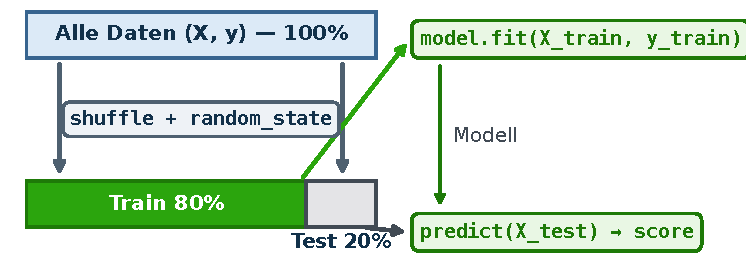
\includegraphics[width=\ZSFgraphicswidth]{Images/machine-learning-train-test-split-workflow.pdf}
\end{center}
\end{contentbox}

% ============================================================
% VORGEGEBENES MODELL
% ============================================================

\subsection{Vorgegebenes Modell einsetzen}\label{sec:09-modell-vorgegeben}
\ZSFkeyword*{Ziel:} Wenn die Aufgabe ein Modell vorgibt, genau diesen \texttt{model}-Block wählen; Split, \texttt{fit}, \texttt{predict} und Bewertung bleiben wie in \ZSFsectionref{sec:09-daten-pruefen}.

\begin{codebox}[DecisionTreeClassifier]
\begin{lstlisting}[style=CodeExpert]
from sklearn.tree import DecisionTreeClassifier
model = DecisionTreeClassifier(
    max_depth=8,                # begrenzt starkes Overfitting
    min_samples_leaf=2,         # robustere Blätter
    random_state=0
)
\end{lstlisting}
\end{codebox}

\begin{codebox}[RandomForestClassifier]
\begin{lstlisting}[style=CodeExpert]
from sklearn.ensemble import RandomForestClassifier
model = RandomForestClassifier(
    n_estimators=200,           # Anzahl Bäume
    max_depth=None,             # kleiner = stärkere Begrenzung
    random_state=0
)
\end{lstlisting}
\end{codebox}

\begin{codebox}[LogisticRegression mit Skalierung]
\begin{lstlisting}[style=CodeExpert]
from sklearn.linear_model import LogisticRegression
from sklearn.pipeline import make_pipeline
from sklearn.preprocessing import StandardScaler

model = make_pipeline(
    StandardScaler(),           # Skalierung gehört ins Modell
    LogisticRegression(max_iter=1000)
)
\end{lstlisting}
\end{codebox}

\begin{codebox}[KNeighborsClassifier mit Skalierung]
\begin{lstlisting}[style=CodeExpert]
from sklearn.neighbors import KNeighborsClassifier
from sklearn.pipeline import make_pipeline
from sklearn.preprocessing import StandardScaler
model = make_pipeline(
    StandardScaler(),           # Distanzen vergleichbar machen
    KNeighborsClassifier(n_neighbors=5)  # Anzahl Nachbarn
)
\end{lstlisting}
\end{codebox}

\begin{codebox}[MLPClassifier mit Skalierung]
\begin{lstlisting}[style=CodeExpert]
from sklearn.neural_network import MLPClassifier
from sklearn.pipeline import make_pipeline
from sklearn.preprocessing import StandardScaler
model = make_pipeline(
    StandardScaler(),           # wichtig für stabiles Training
    MLPClassifier(
        hidden_layer_sizes=(100,),  # robuster Standard: eine Schicht
        max_iter=1000,           # erhöhen, falls keine Konvergenz
        alpha=0.0001,            # grösser = mehr Regularisierung
        random_state=0
    )
)
\end{lstlisting}
\end{codebox}

% ============================================================
% FREIE MODELLWAHL
% ============================================================

\subsection{Alternative: freie Modellwahl}\label{sec:09-modellvergleich}
\ZSFkeyword*{Ziel:} Split aus \ZSFsectionref{sec:09-daten-pruefen} übernehmen, mehrere Modelle gleich trainieren und das Modell mit der höchsten Test-Accuracy wählen.

\begin{codebox}[Modellvergleich: 1. Importe]
\begin{lstlisting}[style=CodeExpert]
from sklearn.tree import DecisionTreeClassifier
from sklearn.ensemble import RandomForestClassifier
from sklearn.linear_model import LogisticRegression
from sklearn.neighbors import KNeighborsClassifier
from sklearn.neural_network import MLPClassifier
from sklearn.pipeline import make_pipeline
from sklearn.preprocessing import StandardScaler
\end{lstlisting}
\end{codebox}

\begin{codebox}[Modellvergleich: 2. Kandidaten-Dict]
\begin{lstlisting}[style=CodeExpert]
# Tree/Forest brauchen keine Skalierung.
# Bei LogReg/KNN/MLP skaliert die Pipeline automatisch.
models = {
    "Tree": DecisionTreeClassifier(
        max_depth=8, min_samples_leaf=2, random_state=0),
    "Forest": RandomForestClassifier(
        n_estimators=200, random_state=0),
    "LogReg": make_pipeline(
        StandardScaler(), LogisticRegression(max_iter=1000)),
    "KNN": make_pipeline(
        StandardScaler(), KNeighborsClassifier(n_neighbors=5)),
    "MLP": make_pipeline(
        StandardScaler(), MLPClassifier(
            hidden_layer_sizes=(100,), max_iter=1000,
            random_state=0))
}
\end{lstlisting}
\end{codebox}

\begin{codebox}[Modellvergleich: 3. Benchmark-Schleife]
\begin{lstlisting}[style=CodeExpert]
from sklearn.metrics import accuracy_score

scores = {}  # Name -> Test-Accuracy

for name, candidate in models.items():  # Alle Modelle durchgehen
    candidate.fit(X_train, y_train)  # Modell trainieren
    predictions = candidate.predict(X_test)  # Testdaten vorhersagen
    scores[name] = accuracy_score(y_test, predictions)  # Accuracy speichern

best_name = max(scores, key=scores.get)  # Key (Name) mit max. Wert
best_model = models[best_name]  # Gewinner-Modell holen
best_accuracy = scores[best_name]  # Beste Accuracy
\end{lstlisting}
\end{codebox}

% ============================================================
% ACCURACY VERBESSERN
% ============================================================

\subsection{Accuracy-Problem erkennen und verbessern}\label{sec:09-accuracy-zu-niedrig}
\ZSFindex{Underfitting}
\ZSFindex{Overfitting}

\begin{codebox}[Train- und Test-Accuracy berechnen]
\begin{lstlisting}[style=CodeExpert]
train_predictions = model.predict(X_train)
train_accuracy = accuracy_score(y_train, train_predictions)

test_predictions = model.predict(X_test)
test_accuracy = accuracy_score(y_test, test_predictions)
\end{lstlisting}
\end{codebox}

\begin{tablebox}[1. Problem an Train- und Test-Accuracy erkennen]
\begin{ZSFtable}[\ZSFfontTableDense]{Y{1.1} Y{0.85} Y{1.05}}
    \ZSFheaderRow
    \ZSFhead{Beobachtung} & \ZSFhead{Problem} & \ZSFhead{Bedeutung} \\
    Training hoch, Test deutlich tiefer & Overfitting & Modell merkt sich Trainingsdaten zu stark. \\
    Training und Test beide tief & Underfitting & Modell erkennt das Muster noch nicht gut genug. \\
    Training und Test beide hoch & kein Problem & Modell generalisiert auf ungesehene Daten. \\
    Ergebnis schwankt stark & instabil & Datensatz klein oder Modell stark vom Split abhängig. \\
\end{ZSFtable}
\end{tablebox}

\begin{tablebox}[2. Beim verwendeten Modell den passenden Parameter ändern]
\begin{ZSFtable}[\ZSFfontTableDense]{Y{0.8} Y{0.75} Y{1.45}}
    \ZSFheaderRow
    \ZSFhead{Modell} & \ZSFhead{Problem} & \ZSFhead{Änderung} \\
    Decision Tree & Overfitting & \texttt{max\_depth} kleiner oder \texttt{min\_samples\_leaf} grösser \\
    Decision Tree & Underfitting & \texttt{max\_depth} grösser \\
    Random Forest & instabil / zu schwach & \texttt{n\_estimators} erhöhen \\
    Logistic Regression & konvergiert nicht & skalieren, \texttt{max\_iter} erhöhen \\
    Logistic Regression & Underfitting & \texttt{C} erhöhen \\
    KNN & Overfitting & \texttt{n\_neighbors} erhöhen \\
    KNN & Underfitting & \texttt{n\_neighbors} verkleinern \\
    MLP & konvergiert nicht & skalieren, \texttt{max\_iter} erhöhen \\
    MLP & Overfitting & \texttt{alpha} erhöhen oder Netz verkleinern \\
    MLP & Underfitting & Netz vergrössern \\
\end{ZSFtable}
\end{tablebox}

% ============================================================
% GRID SEARCH
% ============================================================

\subsection{Alternative: Hyperparameter mit GridSearchCV suchen}\label{sec:09-grid-search}
\ZSFindex{Grid Search}
\ZSFindex{Cross-Validation}
\ZSFkeyword*{Nur verwenden,} wenn die Aufgabe ausdrücklich \texttt{GridSearchCV} oder eine automatische Parametersuche verlangt. Das Beispiel testet passende Werte für einen Decision Tree.

\begin{statementbox}[Merksatz]
\texttt{param\_grid} enthält die Werte, die ausprobiert werden. \texttt{search} wird wie das Modell benutzt: immer zuerst \texttt{fit}, dann \texttt{predict}.
\end{statementbox}

\begin{codebox}[GridSearchCV: Pflichtschema]
\begin{lstlisting}[style=CodeExpert]
from sklearn.model_selection import GridSearchCV
from sklearn.tree import DecisionTreeClassifier

model = DecisionTreeClassifier(random_state=0)  # Basis-Modell

param_grid = {  # Parameter, die ausprobiert werden
    "max_depth": [None, 4, 8],  # Verschiedene Baumtiefen
    "min_samples_leaf": [1, 5]  # Verschiedene Blattgroessen
}

search = GridSearchCV(  # Suche nach besten Parametern konfigurieren
    estimator=model,
    param_grid=param_grid,
    cv=5  # 5 Test-Durchlaeufe (Cross-Validation)
)

search.fit(X, y)  # Alle Kombis testen & beste finden
predictions = search.predict(X_new)  # Vorhersage mit besten Parametern
\end{lstlisting}
\end{codebox}

Siehe Theorie zu Grid Search und Cross-Validation \ZSFref{sec:09-wichtige-parameter}

% ============================================================
% THEORIE UND REFERENZ
% ============================================================

\ZSFmanualColumnBreak
\subsection{Theorie und Modellreferenz}\label{sec:09-theorie}

\subsubsection{Regression vs. Klassifikation}\label{sec:09-ml-typen}
\ZSFindex{Regression}
\ZSFindex[uberwachtes-lernen]{Überwachtes Lernen}
\ZSFindexsee{Supervised Learning}{Überwachtes Lernen}

\begin{factlist}
\ZSFFact{Regression}{sagt einen stetigen Zahlenwert voraus, z.\,B. einen Preis.}
\ZSFFact{Klassifikation}{ordnet einen Datenpunkt einer festen Klasse zu, z.\,B. Spam oder Nicht-Spam.}
\ZSFFact{Supervised Learning}{Training mit Eingaben \texttt{X} und bekannten Zielwerten oder Labels \texttt{y}.}
\ZSFFact{Faustregel}{Zahl mit Einheit oder Skala $\Rightarrow$ Regression; endliche feste Kategorien $\Rightarrow$ Klassifikation.}
\end{factlist}

\begin{tablebox}[Regression oder Klassifikation?]
\begin{ZSFtable}[\ZSFfontTableDense]{Y{1.4} Y{0.6} Y{1.4} Y{0.6}}
    \ZSFheaderRow
    \ZSFhead{Szenario} & \ZSFhead{Typ} & \ZSFhead{Szenario} & \ZSFhead{Typ} \\
    Temperatur morgen & Reg. & Diabetes ja/nein & Klass. \\
    Hauspreis         & Reg. & Betrug ja/nein   & Klass. \\
    Prüfungsnote      & Reg. & Wahrscheinl.\ \% & Reg. \\
\end{ZSFtable}
\end{tablebox}

\subsubsection{Wichtige Parameter}\label{sec:09-wichtige-parameter}
\ZSFindex{Hyperparameter}

\begin{factlist}
\ZSFFact{\texttt{max\_iter}}{Maximale Anzahl Trainingsiterationen; wichtig für \texttt{LogisticRegression}, \texttt{MLPClassifier} und \texttt{MLPRegressor}.}
\ZSFFact{\texttt{hidden\_layer\_sizes}}{Anzahl Neuronen pro versteckter Schicht bei MLP-Modellen.}
\ZSFFact{\texttt{random\_state}}{Fixiert Zufallsprozesse für reproduzierbare Ergebnisse; ist kein Tuning-Parameter für bessere Accuracy.}
\ZSFFact{\texttt{test\_size}}{Anteil der Daten im Testset; üblich sind 0.1 bis 0.3.}
\ZSFFact{\texttt{cv}}{Anzahl Folds bei \texttt{GridSearchCV}; 5 ist ein üblicher Standard.}
\end{factlist}

\begin{contentbox}[Grid Search und K-Fold-Cross-Validation]
\begin{factlist}
\ZSFFact{Grid Search}{probiert vorgegebene Hyperparameter-Kombinationen und vergleicht ihre Scores.}
\ZSFFact{K-Fold}{trainiert das Modell mehrfach; jeder Fold dient einmal als Validierungsmenge. Der Mittelwert schätzt die Modellgüte stabiler als ein einzelner Split.}
\end{factlist}
\end{contentbox}

\begin{contentbox}[K-Fold-Cross-Validation]
\begin{center}
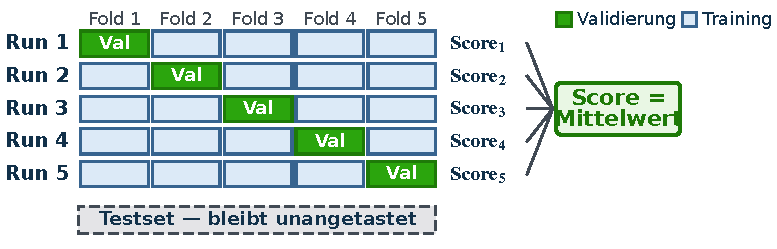
\includegraphics[width=0.56\columnwidth]{Images/machine-learning-k-fold-cross-validation.pdf}
\end{center}
\end{contentbox}

\subsubsection{Klassifikationsmodelle}\label{sec:09-modelle}
\ZSFindex{Logistische Regression}
\ZSFindex{Decision Tree}
\ZSFindex[knn]{KNN / K-Nearest Neighbors}
\ZSFindex{Random Forest}

\begin{contentbox}[Logistic Regression]
\begin{factlist}
\ZSFFact{Idee}{lineare Entscheidungsgrenze; liefert Klassenwahrscheinlichkeiten.}
\ZSFFact{Modell}{Die Wahrscheinlichkeit der positiven Klasse ist
$y=\sigma(w_0+w_1x_1+\cdots+w_nx_n)$.}
\ZSFFact{Schwelle}{Ausgabe ist eine Wahrscheinlichkeit; die Schwelle $0.5$ trennt die Klassen.}
\ZSFFact{Unsicher}{An der Entscheidungsgrenze ist die Vorhersage $\approx0.5$ (maximal unsicher); liegt sie fast überall bei $0.5$, wurde nichts gelernt.}
\ZSFFact{Stärken}{schnell und interpretierbar.}
\ZSFFact{Schwächen}{schwierig bei stark nicht-linearen Mustern; Skalierung ist sinnvoll.}
\ZSFFact{Parameter}{\texttt{C}, \texttt{class\_weight}, \texttt{max\_iter}.}
\end{factlist}
\end{contentbox}

\begin{contentbox}[Decision Tree Classifier]
\begin{factlist}
\ZSFFact{Idee}{zerlegt den Merkmalsraum durch Entscheidungen und sagt in jedem Blatt eine Klasse voraus.}
\ZSFFact{Stärken}{interpretierbar; benötigt keine Skalierung.}
\ZSFFact{Schwächen}{anfällig für Overfitting.}
\ZSFFact{Parameter}{\texttt{max\_depth}, \texttt{min\_samples\_split}, \texttt{min\_samples\_leaf}.}
\end{factlist}
\end{contentbox}

\begin{contentbox}[Random Forest Classifier]
\begin{factlist}
\ZSFFact{Idee}{kombiniert viele zufällig variierte Decision Trees und lässt sie abstimmen.}
\ZSFFact{Stärken}{oft robuster als ein einzelner Tree; benötigt keine Skalierung.}
\ZSFFact{Mehr Bäume}{ein grösseres \texttt{n\_estimators} macht robuster, führt aber \textbf{nicht} zu Overfitting — nur mehr Rechenzeit.}
\ZSFFact{Schwächen}{weniger leicht interpretierbar und rechenintensiver.}
\ZSFFact{Parameter}{\texttt{n\_estimators}, \texttt{max\_depth}, \texttt{min\_samples\_leaf}.}
\end{factlist}
\end{contentbox}

\begin{contentbox}[KNN]
\begin{factlist}
\ZSFFact{Idee}{Klasse durch Mehrheitsentscheid der \texttt{k} nächsten Trainingspunkte.}
\ZSFFact{Kleines k}{flexibel, aber anfällig für Overfitting.}
\ZSFFact{Grosses k}{glatter, kann aber underfitten.}
\ZSFFact{Wichtig}{Features skalieren; \texttt{n\_neighbors} und \texttt{weights} tunen.}
\ZSFFact{Lazy Learning}{kein echtes Training — rechnet erst bei \texttt{predict} alle Distanzen (langsam bei grossen Daten, unzuverlässig in vielen Dimensionen: Fluch der Dimensionalität).}
\ZSFFact{Faustregeln}{$k=n$ ergibt immer die Mehrheitsklasse; ungerades $k$ vermeidet Gleichstände.}
\end{factlist}
\end{contentbox}

\begin{contentbox}[KNN: Einfluss von $k$]
\begin{center}
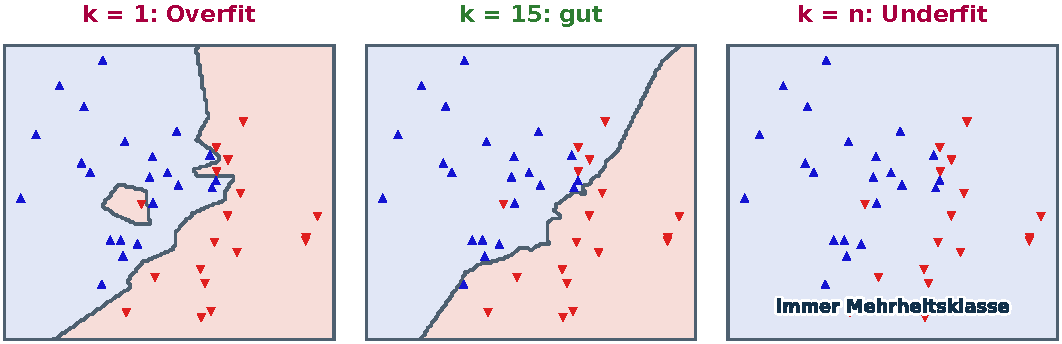
\includegraphics[width=0.62\columnwidth]{Images/machine-learning-knn-k-overfit-underfit-boundaries.pdf}
\end{center}
\end{contentbox}

\begin{contentbox}[MLPClassifier]
\begin{factlist}
\ZSFFact{Idee}{neuronales Netz für nicht-lineare Klassifikationsaufgaben. \ZSFref{sec:10-standard-neural-network-mlp}}
\ZSFFact{Stärken}{flexibel für komplexe Muster.}
\ZSFFact{Schwächen}{mehr Tuning und Rechenzeit; Features skalieren.}
\ZSFFact{Parameter}{\texttt{hidden\_layer\_sizes}, \texttt{activation}, \texttt{alpha}, \texttt{max\_iter}.}
\end{factlist}
\end{contentbox}

\begin{contentbox}[Skalierung: grosse Werte nicht dominieren lassen]
\begin{factlist}
\ZSFFact{Ja}{KNN, MLP, K-Means, PCA — distanz- bzw.\ gradientenbasiert, reagieren auf die Feature-Skala.}
\ZSFFact{Nein}{Decision Tree, Random Forest — arbeiten mit Schwellen-Splits und sind skalenunabhängig.}
\end{factlist}
\end{contentbox}

\subsubsection{Regressionsmodelle}\label{sec:09-regression}
\ZSFindex{Lineare Regression}
\ZSFkeyword*{Ziel des Codes:} Ein Regressionsmodell trainieren und für \texttt{X\_test} stetige Zahlenwerte vorhersagen.

\begin{contentbox}[Linear Regression]
\begin{factlist}
\ZSFFact{Idee}{Vorhersage durch eine lineare Kombination der Eingabefeatures:
$y=w_1x_1+w_2x_2+\cdots+w_nx_n+b$.}
\ZSFFact{Stärken}{schnell, interpretierbar und theoretisch gut verstanden.}
\ZSFFact{Schwächen}{empfindlich gegenüber Ausreissern; kann komplexe Muster nicht abbilden.}
\ZSFFact{Parameter}{\texttt{fit\_intercept} steuert den Bias-Term; \texttt{n\_jobs} die verwendeten CPU-Kerne.}
\ZSFFact{Import}{\texttt{from sklearn.linear\_model import LinearRegression}}
\end{factlist}
\end{contentbox}

\begin{codebox}[LinearRegression]
\begin{lstlisting}[style=CodeExpert]
from sklearn.linear_model import LinearRegression

model = LinearRegression()
model.fit(X_train, y_train)
y_pred = model.predict(X_test)
\end{lstlisting}
\end{codebox}

\begin{contentbox}[Decision Tree Regressor]
\begin{factlist}
\ZSFFact{Idee}{modelliert nicht-lineare Beziehungen durch Entscheidungen an Verzweigungsknoten.}
\ZSFFact{Prinzip}{zerlegt die Eingabemenge in Zonen mit möglichst homogener Zielvariable.}
\ZSFFact{Import}{\texttt{from sklearn.tree import DecisionTreeRegressor}}
\end{factlist}
\end{contentbox}

\begin{contentbox}[Neural Network Regressor]
\begin{factlist}
\ZSFFact{Idee}{neuronales Netz mit Regressionsziel; nicht-linear und flexibel.}
\ZSFFact{Tuning}{\texttt{hidden\_layer\_sizes}, \texttt{max\_iter}, \texttt{activation}.}
\ZSFFact{Import}{\texttt{from sklearn.neural\_network import MLPRegressor}}
\end{factlist}
\end{contentbox}

% ============================================================
% MODELLBEWERTUNG
% ============================================================

\subsection{Modellbewertung und Loss}\label{sec:09-modellbewertung}

\subsubsection{Accuracy und Balanced Accuracy}
\ZSFindex{Accuracy}
\ZSFindex{Balanced Accuracy}
\ZSFindex{Confusion Matrix}

\begin{tablebox}[Binäre Confusion Matrix]
\begin{ZSFtablePlain}{C C C}
\toprule
\ZSFkeyword*{real / vorhergesagt} & \ZSFkeyword*{Positiv} & \ZSFkeyword*{Negativ} \\
\midrule
\ZSFkeyword*{Positiv} & True Pos. (TP) & False Neg. (FN) \\
\ZSFkeyword*{Negativ} & False Pos. (FP) & True Neg. (TN) \\
\bottomrule
\end{ZSFtablePlain}
\end{tablebox}

\begin{formulabox}
\ZSFkeyword*{Accuracy} — Anteil korrekter Klassifikationen:
\[
\text{Accuracy} = \frac{TP + TN}{TP + TN + FP + FN}.
\]
\ZSFgapXS
\ZSFkeyword*{Balanced Accuracy} — Mittelwert der Trefferquoten (binär):
\[
\text{Balanced Accuracy} = \frac{1}{2}(\text{TPR}+\text{TNR}), \qquad
\text{TPR}=\frac{TP}{TP+FN}, \quad
\text{TNR}=\frac{TN}{TN+FP}.
\]
\end{formulabox}

\begin{statementbox}[Mehrere Klassen]
Bei mehreren Klassen ist Balanced Accuracy der Mittelwert des Recalls aller
Klassen. Die Confusion Matrix besitzt dann eine Zeile und Spalte pro Klasse.
\end{statementbox}

\subsubsection{0-1-Loss (Error Rate)}

\begin{contentbox}
Die \ZSFkeyword*{0-1-Loss-Funktion} ist 0 bei einer korrekten und 1 bei einer
falschen Vorhersage:
\[
L(y,\hat y)=
\begin{cases}
0,& y=\hat y,\\
1,& y\neq\hat y.
\end{cases}
\]
Das empirische Risiko ist der Mittelwert
$\frac{1}{n}\sum_{i=1}^n L(y_i,\hat y_i)$. Bei binärer Klassifikation:
\[
\text{Error Rate}=\frac{FP+FN}{TP+TN+FP+FN},
\qquad \text{Accuracy}=1-\text{Error Rate}.
\]
\end{contentbox}

\subsubsection{Gini-Index (Split-Kriterium)}
\ZSFindex{Gini-Index}

\begin{contentbox}
\hl{Intuition:} Der Gini-Index misst, wie gemischt die Klassen in einem Knoten sind: $0$ bedeutet rein (nur eine Klasse), ein grosser Wert bedeutet stark gemischt. Ein Tree bevorzugt Splits mit kleinem Gini-Index, weil ihre Teilmengen klarer einer Klasse zuzuordnen sind.

Die Impurity einer Partition $Part_m$ ist:
\[
G(Part_m)=\sum_k \hat p_{m,k}(1-\hat p_{m,k}).
\]
Für einen Split in $Part_1$ und $Part_2$:
\[
G_{\text{split}}=
\frac{|Part_1|}{|Part_m|}G(Part_1)
+\frac{|Part_2|}{|Part_m|}G(Part_2).
\]
Ein Decision Tree wählt den Split mit kleinem Gini-Index.
\begin{center}
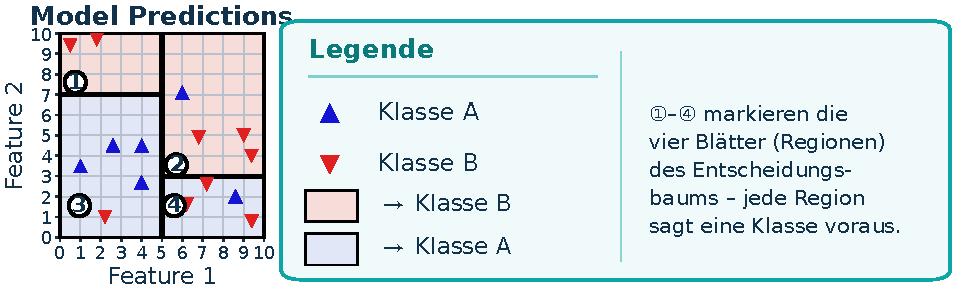
\includegraphics[width=0.73\columnwidth]{Images/decision-tree-gini-split-regions.pdf}
\end{center}
\end{contentbox}

\subsubsection{R2-Score und Mean Squared Error}
\ZSFindex{R2-Score}
\ZSFindex[mse]{MSE / Mean Squared Error}

\begin{formulabox}
Der $R^2$-Score misst die Qualität einer Regressionsvorhersage:
\[
R^2(D,f)=1-\frac{MSE(D,f)}{MSE(D,f_0)}.
\]
\end{formulabox}

\begin{factlist}
\ZSFFact{Lesen}{$R^2=1$: perfekt; $0$: nicht besser als immer den Durchschnitt vorhersagen; $<0$: schlechter.}
\ZSFFact{$f_0$}{konstante Durchschnittsvorhersage.}
\ZSFFact{MSE}{mittlere quadratische Abweichung:
$MSE(D,f)=\frac{1}{n}\sum_{i=1}^n(y_i-\hat y_i)^2$.}
\ZSFFact{MSE vs.\ MAE}{MSE quadriert Fehler, deshalb dominieren Ausreisser (Standardfall). MAE $=\frac{1}{n}\sum_i|y_i-\hat y_i|$ gewichtet linear und ist robust gegen Ausreisser.}
\ZSFFact{Skalierung}{MSE hängt von der Skalierung der Zielwerte ab, $R^2$ nicht.}
\end{factlist}

\subsection{Kategorische Daten encodieren}\label{sec:09-kategorische-daten}
\ZSFindex{Encoding}
\ZSFindex{One-Hot-Encoding}
\ZSFindex{Ordinal Encoding}
\ZSFindex{Mean Encoding}
\ZSFkeyword*{Ziel des Codes:} Kategoriewerte in numerische Spalten umwandeln, bevor sie als Features verwendet werden.

\begin{contentbox}
Maschinelles Lernen erfordert in der Regel numerische Eingabedaten. Nicht-numerische
kategorische Daten wie „Farbe“ oder „Beruf“ müssen zuerst numerisch encodiert werden.
\end{contentbox}

\begin{tablebox}[Encoding-Verfahren im Vergleich]
\begin{ZSFtable}[\ZSFfontTableDense]{Q{0.55} Y{1.2} Y{1.25}}
\toprule
\ZSFkeyword*{Verfahren} & \ZSFkeyword*{Pro} & \ZSFkeyword*{Con} \\
\midrule
Ordinal &
Einfach umsetzbar. Ermöglicht die Abbildung geordneter Kategorien. &
Kann eine falsche Nähe zwischen Kategorien suggerieren und Modellinterpretationen verzerren. \\
\midrule
Mean &
Nutzt den Mittelwert der Zielvariable pro Kategorie und kann nützliche Information übertragen. &
\ZSFdanger{Gefahr von Data Leakage}; erhöhtes Overfitting-Risiko. \\
\midrule
One-hot &
Separate Spalte pro Kategorie; geeignet für nicht-ordinale Kategorien. &
Bei vielen Kategorien entstehen sehr viele Spalten. \\
\bottomrule
\end{ZSFtable}
\end{tablebox}

\begin{codebox}[One-Hot-Encoding mit pandas]
\begin{lstlisting}[style=CodeExpert]
import pandas as pd

pd.get_dummies(a)
\end{lstlisting}
\end{codebox}
